
%% bare_jrnl.tex
%% V1.4b
%% 2015/08/26
%% by Michael Shell
%% see http://www.michaelshell.org/
%% for current contact information.
%%
%% This is a skeleton file demonstrating the use of IEEEtran.cls
%% (requires IEEEtran.cls version 1.8b or later) with an IEEE
%% journal paper.
%%
%% Support sites:
%% http://www.michaelshell.org/tex/ieeetran/
%% http://www.ctan.org/pkg/ieeetran
%% and
%% http://www.ieee.org/

%%*************************************************************************
%% Legal Notice:
%% This code is offered as-is without any warranty either expressed or
%% implied; without even the implied warranty of MERCHANTABILITY or
%% FITNESS FOR A PARTICULAR PURPOSE! 
%% User assumes all risk.
%% In no event shall the IEEE or any contributor to this code be liable for
%% any damages or losses, including, but not limited to, incidental,
%% consequential, or any other damages, resulting from the use or misuse
%% of any information contained here.
%%
%% All comments are the opinions of their respective authors and are not
%% necessarily endorsed by the IEEE.
%%
%% This work is distributed under the LaTeX Project Public License (LPPL)
%% ( http://www.latex-project.org/ ) version 1.3, and may be freely used,
%% distributed and modified. A copy of the LPPL, version 1.3, is included
%% in the base LaTeX documentation of all distributions of LaTeX released
%% 2003/12/01 or later.
%% Retain all contribution notices and credits.
%% ** Modified files should be clearly indicated as such, including  **
%% ** renaming them and changing author support contact information. **
%%*************************************************************************


% *** Authors should verify (and, if needed, correct) their LaTeX system  ***
% *** with the testflow diagnostic prior to trusting their LaTeX platform ***
% *** with production work. The IEEE's font choices and paper sizes can   ***
% *** trigger bugs that do not appear when using other class files.       ***                          ***
% The testflow support page is at:
% http://www.michaelshell.org/tex/testflow/



\documentclass[journal]{IEEEtran}
%
% If IEEEtran.cls has not been installed into the LaTeX system files,
% manually specify the path to it like:
% \documentclass[journal]{../sty/IEEEtran}





% Some very useful LaTeX packages include:
% (uncomment the ones you want to load)


% *** MISC UTILITY PACKAGES ***
%
%\usepackage{ifpdf}
% Heiko Oberdiek's ifpdf.sty is very useful if you need conditional
% compilation based on whether the output is pdf or dvi.
% usage:
% \ifpdf
%   % pdf code
% \else
%   % dvi code
% \fi
% The latest version of ifpdf.sty can be obtained from:
% http://www.ctan.org/pkg/ifpdf
% Also, note that IEEEtran.cls V1.7 and later provides a builtin
% \ifCLASSINFOpdf conditional that works the same way.
% When switching from latex to pdflatex and vice-versa, the compiler may
% have to be run twice to clear warning/error messages.






% *** CITATION PACKAGES ***
%
%\usepackage{cite}
% cite.sty was written by Donald Arseneau
% V1.6 and later of IEEEtran pre-defines the format of the cite.sty package
% \cite{} output to follow that of the IEEE. Loading the cite package will
% result in citation numbers being automatically sorted and properly
% "compressed/ranged". e.g., [1], [9], [2], [7], [5], [6] without using
% cite.sty will become [1], [2], [5]--[7], [9] using cite.sty. cite.sty's
% \cite will automatically add leading space, if needed. Use cite.sty's
% noadjust option (cite.sty V3.8 and later) if you want to turn this off
% such as if a citation ever needs to be enclosed in parenthesis.
% cite.sty is already installed on most LaTeX systems. Be sure and use
% version 5.0 (2009-03-20) and later if using hyperref.sty.
% The latest version can be obtained at:
% http://www.ctan.org/pkg/cite
% The documentation is contained in the cite.sty file itself.






% *** GRAPHICS RELATED PACKAGES ***
%
\ifCLASSINFOpdf
  % \usepackage[pdftex]{graphicx}
  % declare the path(s) where your graphic files are
  % \graphicspath{{../pdf/}{../jpeg/}}
  % and their extensions so you won't have to specify these with
  % every instance of \includegraphics
  % \DeclareGraphicsExtensions{.pdf,.jpeg,.png}
\else
  % or other class option (dvipsone, dvipdf, if not using dvips). graphicx
  % will default to the driver specified in the system graphics.cfg if no
  % driver is specified.
  % \usepackage[dvips]{graphicx}
  % declare the path(s) where your graphic files are
  % \graphicspath{{../eps/}}
  % and their extensions so you won't have to specify these with
  % every instance of \includegraphics
  % \DeclareGraphicsExtensions{.eps}
\fi
% graphicx was written by David Carlisle and Sebastian Rahtz. It is
% required if you want graphics, photos, etc. graphicx.sty is already
% installed on most LaTeX systems. The latest version and documentation
% can be obtained at: 
% http://www.ctan.org/pkg/graphicx
% Another good source of documentation is "Using Imported Graphics in
% LaTeX2e" by Keith Reckdahl which can be found at:
% http://www.ctan.org/pkg/epslatex
%
% latex, and pdflatex in dvi mode, support graphics in encapsulated
% postscript (.eps) format. pdflatex in pdf mode supports graphics
% in .pdf, .jpeg, .png and .mps (metapost) formats. Users should ensure
% that all non-photo figures use a vector format (.eps, .pdf, .mps) and
% not a bitmapped formats (.jpeg, .png). The IEEE frowns on bitmapped formats
% which can result in "jaggedy"/blurry rendering of lines and letters as
% well as large increases in file sizes.
%
% You can find documentation about the pdfTeX application at:
% http://www.tug.org/applications/pdftex





% *** MATH PACKAGES ***
%
%\usepackage{amsmath}
% A popular package from the American Mathematical Society that provides
% many useful and powerful commands for dealing with mathematics.
%
% Note that the amsmath package sets \interdisplaylinepenalty to 10000
% thus preventing page breaks from occurring within multiline equations. Use:
%\interdisplaylinepenalty=2500
% after loading amsmath to restore such page breaks as IEEEtran.cls normally
% does. amsmath.sty is already installed on most LaTeX systems. The latest
% version and documentation can be obtained at:
% http://www.ctan.org/pkg/amsmath





% *** SPECIALIZED LIST PACKAGES ***
%
%\usepackage{algorithmic}
% algorithmic.sty was written by Peter Williams and Rogerio Brito.
% This package provides an algorithmic environment fo describing algorithms.
% You can use the algorithmic environment in-text or within a figure
% environment to provide for a floating algorithm. Do NOT use the algorithm
% floating environment provided by algorithm.sty (by the same authors) or
% algorithm2e.sty (by Christophe Fiorio) as the IEEE does not use dedicated
% algorithm float types and packages that provide these will not provide
% correct IEEE style captions. The latest version and documentation of
% algorithmic.sty can be obtained at:
% http://www.ctan.org/pkg/algorithms
% Also of interest may be the (relatively newer and more customizable)
% algorithmicx.sty package by Szasz Janos:
% http://www.ctan.org/pkg/algorithmicx




% *** ALIGNMENT PACKAGES ***
%
%\usepackage{array}
% Frank Mittelbach's and David Carlisle's array.sty patches and improves
% the standard LaTeX2e array and tabular environments to provide better
% appearance and additional user controls. As the default LaTeX2e table
% generation code is lacking to the point of almost being broken with
% respect to the quality of the end results, all users are strongly
% advised to use an enhanced (at the very least that provided by array.sty)
% set of table tools. array.sty is already installed on most systems. The
% latest version and documentation can be obtained at:
% http://www.ctan.org/pkg/array


% IEEEtran contains the IEEEeqnarray family of commands that can be used to
% generate multiline equations as well as matrices, tables, etc., of high
% quality.




% *** SUBFIGURE PACKAGES ***
%\ifCLASSOPTIONcompsoc
%  \usepackage[caption=false,font=normalsize,labelfont=sf,textfont=sf]{subfig}
%\else
%  \usepackage[caption=false,font=footnotesize]{subfig}
%\fi
% subfig.sty, written by Steven Douglas Cochran, is the modern replacement
% for subfigure.sty, the latter of which is no longer maintained and is
% incompatible with some LaTeX packages including fixltx2e. However,
% subfig.sty requires and automatically loads Axel Sommerfeldt's caption.sty
% which will override IEEEtran.cls' handling of captions and this will result
% in non-IEEE style figure/table captions. To prevent this problem, be sure
% and invoke subfig.sty's "caption=false" package option (available since
% subfig.sty version 1.3, 2005/06/28) as this is will preserve IEEEtran.cls
% handling of captions.
% Note that the Computer Society format requires a larger sans serif font
% than the serif footnote size font used in traditional IEEE formatting
% and thus the need to invoke different subfig.sty package options depending
% on whether compsoc mode has been enabled.
%
% The latest version and documentation of subfig.sty can be obtained at:
% http://www.ctan.org/pkg/subfig




% *** FLOAT PACKAGES ***
%
%\usepackage{fixltx2e}
% fixltx2e, the successor to the earlier fix2col.sty, was written by
% Frank Mittelbach and David Carlisle. This package corrects a few problems
% in the LaTeX2e kernel, the most notable of which is that in current
% LaTeX2e releases, the ordering of single and double column floats is not
% guaranteed to be preserved. Thus, an unpatched LaTeX2e can allow a
% single column figure to be placed prior to an earlier double column
% figure.
% Be aware that LaTeX2e kernels dated 2015 and later have fixltx2e.sty's
% corrections already built into the system in which case a warning will
% be issued if an attempt is made to load fixltx2e.sty as it is no longer
% needed.
% The latest version and documentation can be found at:
% http://www.ctan.org/pkg/fixltx2e


%\usepackage{stfloats}
% stfloats.sty was written by Sigitas Tolusis. This package gives LaTeX2e
% the ability to do double column floats at the bottom of the page as well
% as the top. (e.g., "\begin{figure*}[!b]" is not normally possible in
% LaTeX2e). It also provides a command:
%\fnbelowfloat
% to enable the placement of footnotes below bottom floats (the standard
% LaTeX2e kernel puts them above bottom floats). This is an invasive package
% which rewrites many portions of the LaTeX2e float routines. It may not work
% with other packages that modify the LaTeX2e float routines. The latest
% version and documentation can be obtained at:
% http://www.ctan.org/pkg/stfloats
% Do not use the stfloats baselinefloat ability as the IEEE does not allow
% \baselineskip to stretch. Authors submitting work to the IEEE should note
% that the IEEE rarely uses double column equations and that authors should try
% to avoid such use. Do not be tempted to use the cuted.sty or midfloat.sty
% packages (also by Sigitas Tolusis) as the IEEE does not format its papers in
% such ways.
% Do not attempt to use stfloats with fixltx2e as they are incompatible.
% Instead, use Morten Hogholm'a dblfloatfix which combines the features
% of both fixltx2e and stfloats:
%
% \usepackage{dblfloatfix}
% The latest version can be found at:
% http://www.ctan.org/pkg/dblfloatfix




%\ifCLASSOPTIONcaptionsoff
%  \usepackage[nomarkers]{endfloat}
% \let\MYoriglatexcaption\caption
% \renewcommand{\caption}[2][\relax]{\MYoriglatexcaption[#2]{#2}}
%\fi
% endfloat.sty was written by James Darrell McCauley, Jeff Goldberg and 
% Axel Sommerfeldt. This package may be useful when used in conjunction with 
% IEEEtran.cls'  captionsoff option. Some IEEE journals/societies require that
% submissions have lists of figures/tables at the end of the paper and that
% figures/tables without any captions are placed on a page by themselves at
% the end of the document. If needed, the draftcls IEEEtran class option or
% \CLASSINPUTbaselinestretch interface can be used to increase the line
% spacing as well. Be sure and use the nomarkers option of endfloat to
% prevent endfloat from "marking" where the figures would have been placed
% in the text. The two hack lines of code above are a slight modification of
% that suggested by in the endfloat docs (section 8.4.1) to ensure that
% the full captions always appear in the list of figures/tables - even if
% the user used the short optional argument of \caption[]{}.
% IEEE papers do not typically make use of \caption[]'s optional argument,
% so this should not be an issue. A similar trick can be used to disable
% captions of packages such as subfig.sty that lack options to turn off
% the subcaptions:
% For subfig.sty:
% \let\MYorigsubfloat\subfloat
% \renewcommand{\subfloat}[2][\relax]{\MYorigsubfloat[]{#2}}
% However, the above trick will not work if both optional arguments of
% the \subfloat command are used. Furthermore, there needs to be a
% description of each subfigure *somewhere* and endfloat does not add
% subfigure captions to its list of figures. Thus, the best approach is to
% avoid the use of subfigure captions (many IEEE journals avoid them anyway)
% and instead reference/explain all the subfigures within the main caption.
% The latest version of endfloat.sty and its documentation can obtained at:
% http://www.ctan.org/pkg/endfloat
%
% The IEEEtran \ifCLASSOPTIONcaptionsoff conditional can also be used
% later in the document, say, to conditionally put the References on a 
% page by themselves.




% *** PDF, URL AND HYPERLINK PACKAGES ***
%
%\usepackage{url}
% url.sty was written by Donald Arseneau. It provides better support for
% handling and breaking URLs. url.sty is already installed on most LaTeX
% systems. The latest version and documentation can be obtained at:
% http://www.ctan.org/pkg/url
% Basically, \url{my_url_here}.




% *** Do not adjust lengths that control margins, column widths, etc. ***
% *** Do not use packages that alter fonts (such as pslatex).         ***
% There should be no need to do such things with IEEEtran.cls V1.6 and later.
% (Unless specifically asked to do so by the journal or conference you plan
% to submit to, of course. )


% correct bad hyphenation here
\hyphenation{op-tical net-works semi-conduc-tor}
\usepackage{graphicx}
\usepackage[table,xcdraw]{xcolor}
\usepackage[TABBOTCAP]{subfigure}
\usepackage{bm}
\usepackage{upgreek} 
\usepackage{amsmath}
\usepackage{breqn}
\usepackage{color}
\usepackage{cite}
\usepackage[none]{hyphenat}
\usepackage{algorithm}
\usepackage{algorithmic}
\usepackage{amssymb}

\usepackage{multirow}


% Neurocomputing
\usepackage{float}
\usepackage{caption}
\usepackage{array}
\usepackage{booktabs}
% 设置超链接跳转
\usepackage[colorlinks,
linkcolor=blue,
anchorcolor=blue,
citecolor=blue]{hyperref} 
\usepackage{amsmath}

% 改变字体颜色
\usepackage{color,xcolor}
\usepackage{makecell}

% 智能引用
%\usepackage{hyperref}
%\usepackage{cleveref}
%
%% 跨文件引用
\usepackage{xr}
\externaldocument{figs/prediction_accuracies}

% include文件不分页
%\usepackage{newclude}

% 给表格添加注脚
\usepackage{threeparttable}
\usepackage{footnote}



\begin{document}
%
% paper title
% Titles are generally capitalized except for words such as a, an, and, as,
% at, but, by, for, in, nor, of, on, or, the, to and up, which are usually
% not capitalized unless they are the first or last word of the title.
% Linebreaks \\ can be used within to get better formatting as desired.
% Do not put math or special symbols in the title.
\title{BAN: Neuroanatomical Aligning in Auditory Recognition between Deep Neural Network and Human Brain}
%
%
% author names and IEEE memberships
% note positions of commas and nonbreaking spaces ( ~ ) LaTeX will not break
% a structure at a ~ so this keeps an author's name from being broken across
% two lines.
% use \thanks{} to gain access to the first footnote area
% a separate \thanks must be used for each paragraph as LaTeX2e's \thanks
% was not built to handle multiple paragraphs
%


\author{Haidong~Wang, Zhiyong Li, \emph{Member, IEEE},~Xuan He,~Ke Nai,~and Ming Wen% <-this % stops a space
	\thanks{H. Wang, Z. Li, K. Nai, S. Wang and J. Lv are with the School
		of Computer Science and Electronic Engineering of Hunan University, Key Laboratory for Embedded and Network Computing of Hunan Province, Changsha 410082,
		China (e-mail: haidong\_hnu@hnu.edu.cn; zhiyong.li@hnu.edu.cn;
		naike@hnu.edu.cn).}
	\thanks{M. Wen is with State Grid Hunan Electric Power Company Limited Economical \& Technical Research Institute, Hunan Key Laboratory of Energy Internet Supply-demand and Operation, Changsha 410000, China (e-mail: hnjyy1903wen@126.com).}
% % <-this % stops a space
}


% note the % following the last \IEEEmembership and also \thanks - 
% these prevent an unwanted space from occurring between the last author name
% and the end of the author line. i.e., if you had this:
% 
% \author{....lastname \thanks{...} \thanks{...} }
%                     ^------------^------------^----Do not want these spaces!
%
% a space would be appended to the last name and could cause every name on that
% line to be shifted left slightly. This is one of those "LaTeX things". For
% instance, "\textbf{A} \textbf{B}" will typeset as "A B" not "AB". To get
% "AB" then you have to do: "\textbf{A}\textbf{B}"
% \thanks is no different in this regard, so shield the last } of each \thanks
% that ends a line with a % and do not let a space in before the next \thanks.
% Spaces after \IEEEmembership other than the last one are OK (and needed) as
% you are supposed to have spaces between the names. For what it is worth,
% this is a minor point as most people would not even notice if the said evil
% space somehow managed to creep in.



% The paper headers
\markboth{Journal of \LaTeX\ Class Files,~Vol.~14, No.~8, August~2015}%
{Shell \MakeLowercase{\textit{et al.}}: Bare Demo of IEEEtran.cls for IEEE Journals}
% The only time the second header will appear is for the odd numbered pages
% after the title page when using the twoside option.
% 
% *** Note that you probably will NOT want to include the author's ***
% *** name in the headers of peer review papers.                   ***
% You can use \ifCLASSOPTIONpeerreview for conditional compilation here if
% you desire.




% If you want to put a publisher's ID mark on the page you can do it like
% this:
%\IEEEpubid{0000--0000/00\$00.00~\copyright~2015 IEEE}
% Remember, if you use this you must call \IEEEpubidadjcol in the second
% column for its text to clear the IEEEpubid mark.



% use for special paper notices
%\IEEEspecialpapernotice{(Invited Paper)}




% make the title area
\maketitle

% As a general rule, do not put math, special symbols or citations
% in the abstract or keywords.
\begin{abstract}
Inspired by neuroanatomy, deep neural networks (DNNs) have recently developed from shallow network structures to exceedingly deep structures, providing excellent recognition performance.
However, standard DNNs usually do not easily connect with brain areas on account of their excessive network depth and absent biological constraints, such as recurrent connections. 
We propose a brain-like auditory network (BAN) with four neuroanatomically mapped regions and recurrence, guided by the brain-like auditory score (BAS), 
a novel benchmark to measure the model similarity of the human smooth pursuit pathway. 
In addition, we propose that the middle temporal (MT) and medial superior temporal (MST) areas in the cerebral cortex are equivalent to the designed network structure on the basis of the continuous motion perception of the tracking pathway, 
and indicate that the metrics between the neuroanatomical similarity in the cerebral cortex and visual tracking of the DNN are compatible. 
Despite having significant tracking performance on the Tracking-Gump dataset, the BTN has achieved a high BTS. 
In summary, this research builds a BTN, a brain-like and recurrent DNN, as the first model of the cortical pathway of smooth pursuit.
\end{abstract}

% Note that keywords are not normally used for peerreview papers.
\begin{IEEEkeywords} 
Online Multi-object Tracking, End-to-end Model, Joint Detection and Data Association. 
\end{IEEEkeywords}


% For peer review papers, you can put extra information on the cover
% page as needed:
% \ifCLASSOPTIONpeerreview
% \begin{center} \bfseries EDICS Category: 3-BBND \end{center}
% \fi
%
% For peerreview papers, this IEEEtran command inserts a page break and
% creates the second title. It will be ignored for other modes.
\IEEEpeerreviewmaketitle



\begin{figure*}
	\centering
	\includegraphics[width=6.7in]{figs/introduction.pdf}
	\caption{
		\textbf{
		Collaborative design between a DNN and neuroanatomy with a BAS.} 
		Through the quantitative brain-like score, we refer to the human brain and utilize acquired knowledge to enlighten the design of the BTN. 
		The BAN includes four regions that are mapped into the primary auditory cortex (A1), 		the belt or peripheral area, parabelt cortex (PB) and the areas of temporal cortex (T2/T3). 
		CONV\textsubscript{V1} is the classical convolutional layer and performs preprocessing to reduce the data size.
		The DFN\textsubscript{MT/MST} is dynamic filter network, and the RNN\textsubscript{FEF} is recurrent, as depicted in Section~\ref{sec:cornet_s_def} for details.
		The the upper-right image corresponds to the tracking activation and bounding box in the brain-aligned models, 
		while lower-right image represents the cortical activation and eye gaze position with the stimulus in the far left,
		which demonstrates the relationship between computer vision tracking performance and brain tracking response with the BTS, as depicted in Section~\ref{sec:experiments}.
	}
	\label{fig:introduction}
\end{figure*}


\section{Introduction}
% The very first letter is a 2 line initial drop letter followed
% by the rest of the first word in caps.
% 
% form to use if the first word consists of a single letter:
% \IEEEPARstart{A}{demo} file is ....
% 
% form to use if you need the single drop letter followed by
% normal text (unknown if ever used by the IEEE):
% \IEEEPARstart{A}{}demo file is ....
% 
% Some journals put the first two words in caps:
% \IEEEPARstart{T}{his demo} file is ....
% 
% Here we have the typical use of a "T" for an initial drop letter
% and "HIS" in caps to complete the first word.+

% problem: time, optimization joint
% the development of object detection
% joint detection and embeding, -> problem
% joint detection and association
% contribution: end-to-end, data preparation, training

% /data3/dong/data/brain/auditory/Music_Genre_Classification_Pytorch-master/report.pdf, 1. Music
\IEEEPARstart{M}{usic} genres are a set of descriptive keywords that convey high-level information about a music clip (jazz, classical and rock .etc).
Genre classification is a task that aims to predict music genre using audio signal.
According to Tzanetakis and Cook~\cite{tzanetakis2002musical}, the genre of music is a categorical label created by humans to characterize musical works.
The genre of music is characterized by a common characteristic shared by members.
These characteristics are typically associated with musical instruments, rhythmic structures and harmonized content.
Automatic music genre classification can help or replace human users in the process and will be a valuable addition to the music information retrieval system.
According to Nam~\cite{nam2018deep}, music genre classification has a significant impact on music search and recommendation of music streaming services.
In the above mentioned musical classification and tagging task solving methodology, it is very important to make the computer aware of the pattern of music and identify them.
The characteristics of this traditional framework are critical to the design of pipeline through feature engineering and classifier production.

When humans distinguish music, it is important to tell machines the feature inside the music, just they distinguish genres through the sound of musical instruments or through rhythm.
This is commonly called hand engineering using domain knowledge.
But as we move on to the era of deep learning after 2015, a variety of attempts and high performance begin to emerge.
The deep learning methodology leverages less domain knowledge and allows feature learning.
In general, the deep learning methodology builds pipeline through linear part, line transformation, nonlinear part activation function, and optional pooling operation.
As you pass through these layers, the model learns feature and enables end-to-end learning.


Deep learning has made great progress in building the candidate model of the neuromechanism in the neurological community~\cite{kubilius2019brain-like}. 
Amazingly, in trained deep neural networks (DNNs) used to classify images~\cite{Deng2009ImageNet}, the middle layer in DNNs can partially explain why the nerve cell in the middle layer of the visual cortex has specific activations to an image~\cite{yamins2014performance,khaligh2014deep,gucclu2015deep,murugesan2017brain,cichy2016deep,yamins2016using}. 
Furthermore, these models also partly predict primate image recognition behavior and cortical activation~\cite{rajalingham2018large,kubilius2016deep}.
Excellent models of the brain provide extraordinary opportunities for brain-computer interfaces,
and these methods can be utilized to predict the expected activations in the cortical pathway~\cite{bashivan2019neural}.


To capture cortical processing even more strictly in these models, continued architectural search on traditional visual datasets alone no longer seems to be a feasible solution. 
Even though the great tracking performance in deeper DNNs has truly increased~\cite{ILSVRC15,luo2021trajectory}, it is hopeless to raise the brain-like score~\cite{rajalingham2018large,su2020incremental}. 
In addition, at the beginning, only partial modules can be obviously mapped to corresponding regions of the visual pathway, 
and the relations between the small number of visual regions and the numerous and complex modules in GoogleNet~\cite{szegedy2015going} or Inception-v4~\cite{szegedy2017inception} are inconspicuous. 
Finally, the network with high accuracy in the visual task becomes increasingly deeper except for several brain-like architectures for image classification~\cite{TangSchrimpfLotter2018Recurrent, kar2019evidence}. 


To address the interpretability problem of visual tracking model, in this study, we propose that aligning DNNs to anatomy will result in shallower, more interpretable, and more brain-like tracking models, named brain-like tracking network (BTN).
The BTN is a shallow recurrent brain-like architecture of the brain pathway; 
hence, it has a much more brain-like structure. 
In section 4, we introduce the method utilized to analyse human behavioral and cortical data during object tracking. 
In section 5, we build a fancy measurement method for predicting eye movement behavior and neural activations on the brain-like tracking score (BTS). 
In our experiments, we introduce a new benchmark dataset composed of behavioral and cortical recordings, 
and present an outstanding tracking result of 36.5\% at evaluating the model similarity of the visual pathway while obtaining a good tracking effect in the Tracking-Gump dataset~\cite{gaze_forrest}. 
We find that these results are mainly due to the brain-like architecture, in accordance with prior knowledge of the human cortical pathway processing stimuli input~\cite{TangSchrimpfLotter2018Recurrent, yin2020deep, kar2019evidence}. 
Finally, to compare the model activations between the RNN\textsubscript{MT/MST} in the BTN and the responses in the human middle temporal and medial superior temporal areas (MT/MST), we discover that the BTN predicts these cortical activations well, 
and it is also the first visual tracking model to do so on the neural recordings. 

% You must have at least 2 lines in the paragraph with the drop letter
% (should never be an issue)

\section{Related Works} 

\subsection{Deep neural network}\par
Many works have recently shown that salient objects are extracted by a series of foveal views~\cite{mnih2014recurrent,draw}.
The object extraction module in the BTN is implemented with a two-dimensional gaussian filter~\cite{RATM} that is neuroanatomically explainable.
Focusing on specific appearance representations may be as important as spatial attention. 
An approach with recurrence can adaptively change the filter of the convolution module, therefore changing it to presentations on a frame and optimizing model performance~\cite{stollenga2014deep}. 
The filters of the dynamic filter network (DFN)~\cite{brabandere2016dynamic} are obtained online based on the input feature, and the DFN implements model compression without degrading the accuracy. 
Input-dependent state transitions can help to learn the markovian decision model~\cite{karl2017deep}. 
\textcolor{red}{
	We do not follow the results, and use the idea to predict the salient feature.} 


\textcolor{red}{
	To track a target, it seems to be very suitable to use recurrences and glimpses, but they have only been employed successfully in monochromatic videos with simple backgrounds~\cite{RATM}. 
	Some~\cite{ning2017spatially} obtained prominent results through representations of the target detector that is the input of a recurrent neural network (RNN)~\cite{su2020improved}.
	However, it needs to process each full frame. 
	A recent study~\cite{gordon2017re3} utilized an RNN cropping explicitly to build attention in humans. 
	Our study is similar to~\cite{RATM,luo2019teleoperation}, and utilizes human attention which is implemented with a long short memory network (LSTM) to extract the movement features well in multiple frames. 
	In addition, we seek to design a brain-like network that will gain a superior BTS and exceed the existing tracking models on the Tracking-Gump dataset~\cite{gaze_forrest}.
}\par

\subsection{Smooth pursuit}
There have been many successful eye movement experiments. 
Some eye movement detection methods are proposed according to the existing plentiful datasets that have annotated eye movement data~\cite{dorr2010variability,mathe2012dynamic,hooge2017is,blstm_class}. 
Many of the existing classification methods, which are designed using motionless input, only process saccades and fixations. 
Therefore, these methods cannot detect smooth pursuit and prevent the detection of brain-like correlations with smooth pursuit. 
In order to address this issue, a multi-observer smooth pursuit method (MOSP)~\cite{mosp} that can differentiate three primary eye movements, including saccade, fixation and smooth pursuit, 
and acquire good performance evaluation is designed~\cite{blstm_class}.
In addition, to accurately explain the domain of  intelligence as a brain-like model in the human brain and cognitive sciences, 
the brain-score has been proposed in the research of an integrated benchmark in the field of computer vision~\cite{schrimpf2020integrative}. 

In this work, we take full advantage of the latest achievements. 
By utilizing these excellent eye movement classification and computer vision methods, 
we can process functional magnetic resonance imaging (fMRI) and gaze data in the studyforrest dataset~\cite{gaze_forrest} 
and detect corresponding cortical regions associated with saccadic and smooth pursuit in Tracking-Gump.
In addition, based on model activation and cortical activation, we designed the BTS to measure their similarity.


\section{BAN: Brain-like Auditory Network} 
In this section, we introduce the proposed BTN with three steps. 
First, we indicate the motivation and design criteria in our methods.
Second, we detail each component in the BTN pipeline. 
Finally, we introduce the loss function to train the BTN. \par

\subsection{Design criteria}
Our aim is to obtain a high brain-likeness between visual object tracking in DNN and the smooth pursuit in brain.
Additionally, smooth-pursuit movements in our brain keep the image of a moving target on the fovea. 
\textcolor{red}{
	In the pathway of smooth pursuit,
	primary visual cortex (V1) is the first stage to preprocess the input signals, 
	MT/MST \textcolor{red}{integrate} motion signal across space,
	and frontal eye field (FEF) generates predictive eye movement signals~\cite{b11,b13,b14}.
}\par

\textcolor{red}{
	Inspired by the pathway of smooth pursuit in brain, we build neuroanatomical mapping from cortical regions to DNN layers, as depicted in Figure~\ref{fig:introduction}.}
For model comparison, we build the mapping by examining the layer in the DNN that understands activations well in a specific cortical region, 
ideally such activations will already be predicted by the model with no superfluous parameters. 
Therefore, the BTN consists of four neural network modules including convolution layer, DFN, LSTM and FC.
And they are the analogy to the smooth pursuit pathway V1, MT/MST, FEF, 
and motion predictor that converts the output of FEF to corresponding motion responses, as depicted in Figure~\ref{fig:pipeline}. 
This plain idea of explicit brain areas segmentation is an important step to design a brain-like tracking model, 
and we are committed to finding more universal structures. 
Examples include an entire model as a neural network with no difference in cortical areas
and various connections that may improve BTS in future work.
In addition, we follow these two criteria to design the BTN~\cite{kubilius2018predict}:

(1) \textbf{Architecture}: In models with similar tracking performance, we prefer a brain-like network because it is easier to understand and can meet the anatomical constraints.
And we use DNNs because their neurons are the basic unit of data processing, 
and all neural activations in DNNs can be clearly mapped to cortical activation~\cite{yamins2016using}.
\textcolor{red}{
	In addition, recurrent connections are naturally considered for visual object tracking on account of the temporal attributes in the video sequence.}
Activations in the dorsal pathway also have a temporal attribute; 
therefore, the BTN is assumed to generate activations in time series.

(2) \textbf{Predictivity}: 
There is more correct behavior output in intermediate layers and final outputs that meet neuroanatomical constraints (neural responses). 
This make our model have an ability to predict cortical activation and human eye movement behavior.

We now introduce the pipeline for BTN. 


\subsection{BTN pipeline} \label{sec:cornet_s_def}

Given the input frame $F_t$ and attention parameters $a_t$, the fovea (imitating spatial attention) selects a foveal view $f_t$. 
\textcolor{red}{Moreover, we use an appearance selector, parameterized with appearance $\alpha _t$ including V1 and this dorsal pathway and ventral pathway, to obtain the tracked target representations $m_t$ 
	and update hidden state $h_t$ in LSTM.}
Then, we decode the output of LSTM and use it to infer the eye movement $\Delta p_t$, spatial attention $a_{t+1}$ and the appearance attention $\alpha _{t+1}$ in the next frame.  
Appearance attention is driven by top-down information $\alpha _t$ and bottom-up (the foveal view $f_t$) information. 
However, spatial attention only relies on top-down information $a_t$.
In this case, bottom-up information only has localized impacts and relies on salience input at a position, 
but top-down information combines global features into localized analysis. 
The attention mechanism, which intensified with recurrence, imitates the visual cortex~\cite{attention}.
Then, we detail each component of the brain-like tracking architecture. 


%\begin{figure*}
%	\centering
%	\includegraphics[width=5.7in]{figs/pipeline.pdf}
%	\caption{
	%		\textbf{
		%			The designed architecture in visual object tracking in humans.} 
	%		The believable cortical areas implementing particular roles in smooth pursuit are indicated with rectangular modules.
	%		The foveal view $f_t$ is obtained in the input frame $F_t$ with the spatial selector in the fovea. 
	%		V1 and the ventral pathway learn the appearance representations $v_t$, 
	%		and neurons in the dorsal pathway (including V1 and MT/MST) segment the salient object $d_t$ and background on the foveal view.
	%		The refined representations $m_t$ are utilized to compute the working memory $h_t$.
	%		Specifically, the FEF may be more important for initiating pursuit learning based on the target velocity,
	%		and we combine FEF output $o_t$ and dorsal stream output $d_t$ into the next module. 
	%		The cerebellum and brainstem together (including pontine nuclei (PN), flocculus, vermis and vestibular nuclei (VN)) are modeled by fully connected layers (FCs) to generate attention $a_{t+1}$, appearance $\alpha_{t+1}$, and eye position correction signals $\Delta p$,
	%		even the final eye movement ($\Delta p_t$) via the oculomotor.
	%		All black arrows indicate that information flows within one time-step, 
	%		while the gray colored arrows represent the temporal connections.  
	%	}
%	\label{fig:pipeline}
%\end{figure*}

\subsubsection{Retina and Dorsal/Ventral \textcolor{red}{Pathway}}
Typical, input is a data matrix represented by a time-frequency representation. 
Typically there is a Mel-spectrogram.

The spatial selector selects the foveal view $f_t$ for the current frame $F_t$,
and its output is transmitted to two interconnected cortical pathways.
The ventral pathway recognizes the tracked targets 
and the dorsal pathway learns motion features in the field of view. 
\textcolor{red}{
	We present the dorsal pathway with the MT/MST that analyses motion features, as depicted in Figure~\ref{fig:pipeline};
	and computes a foreground segmentation $d_t$ of the foveal view.}

(1) \textbf{Retina}: 
The spatial attention mechanism in our model pipeline is modeled according to~\cite{RATM}. 
An input frame $F_t \in R^{W \times H}$ forms matrices $M_t^x \in R^{w \times W}$ and $M_t^y \in R^{h \times H}$.
A row of the matrix contains a gaussian distribution. 
The position and width of the gaussian distribution determine which parts of the input frame are selected as the foveal view $f_t$ in the retina.
Therefore, the foveal view $f_t \in R^{h \times w}$ can be denoted as
\begin{equation}
	f_t = M_t^y F_t (M_t^x)^T.
\end{equation}
We represent attention with the distributive center, the variance and the stride of the distributive center of continuous matrix rows.
Unlike the study~\cite{hart}, only the stride and center are predicted through LSTM;
however, variance only relies on stride.
The operation avoids extravagant bias when estimating a smaller variance, contributing to a faster learning speed. 
In addition, the utilized size of $f_t$ relies on the experimental analysis. 

(2) \textbf{Ventral Pathway}: 
The ventral pathway converts the foveal view $f_t$ into a fixed dimension vector $v_t$ including spatial and appearance features of the tracked object. 
The network structure architecture relies on the specific experimental analysis. 
In the architecture of the ventral pathway, we implement V1 using a CNN, which is a mutual module in the ventral pathway and dorsal pathway.
Generally, however, we implement V1 using several convolutional layers and max pooling layers. 
\textcolor{red}{
	These layers, which imitate V1 in humans~\cite{theoretical_neuroscience}, are shared with the dorsal pathway.}
In addition, the pipeline is split into dorsal and ventral pathways. 
Finally, we implement the ventral pathway by CNN that extracts object representations $v_t$.

(3) \textbf{Dorsal Pathway}: 
The dorsal pathway (MT/MST) is implemented as a DFN~\cite{brabandere2016dynamic} 
and is used to address spatial relations between the foreground and background. 
Let FC$(\cdot)$ indicate a fully connected layer.
MT/MST utilizes appearance representation $\alpha_t$ to dynamically predict the convolutional filter $\phi_t$
\begin{equation}
	\left\{ \phi _t ^i \right\}_{i=1}^N = \text{FC}(\alpha_t).
\end{equation}
The filters with corresponding nonlinearities in $N$ convolutional layers are applied to the feature in V1. 
Then, we apply a $1 \times 1$ convolution and a sigmoid function to convert the representation into a two-dimensional mask $d_t$.
\textcolor{red}{
	Every point in $d_t$ indicates how likely the pursued target is occupied.}

The position map of the dorsal pathway is integrated over the object representations learned by the ventral pathway, which simulate the noise restraining mechanism in the visual system. 
This can handle occlusion and avoid drift, because the target representation is not overwritten in LSTM when the current frame has no representations of the pursued target. 
Therefore, the output of ventral and dorsal pathways are integrated as
\begin{equation}
	m_t = \text{FC}(conc(v_t \odot d_t)),
\end{equation}
where $\odot$ indicates the Hadamard product that performs salient object extraction through the representation mask, 
and $conc$ means a concatenation operator that concatenates all rows of a matrix into a vector.

\subsubsection{FEF}

The proposed method depends on the ability to estimate the object appearance and position in the next frame; 
and therefore, it heavily relies on state prediction. 
The LSTM can utilize spatial-temporal and appearance features, 
and enables the proposed model to handle occlusion and drifting target representations, such as a tracked \textcolor{red}{target} obscured by other distractors. 

The LSTM module, presented in Figure~\ref{fig:pipeline} and named the FEF, utilizes \textcolor{red}{the} output error to predict eye movement. 
Similar predictive actions exist when smooth pursuit is demonstrated in the FEF area that accepts the output of the dorsal stream~\cite{b11,b13,b14}. 
The output error goes to zero when the delay between object and eye movement is decreased in model training; 
thus, LSTM requires inferring eye motion without image input.
The refined representations $m_t$ are used to update the hidden state $h_t$ in the FEF. 
\begin{equation} \label{LSTM}
	h_t, o_t = \text{LSTM}(h_{t-1}, m_t).
\end{equation}



\subsubsection{Brainstem/Cerebellum}

Then we utilize the output $d_t$ and $o_t$ to estimate eye movement $\Delta p_t$, attention $a_{t+1}$ and appearance $\alpha_{t+1}$.
\begin{equation} \label{FC}
	\Delta p_t, \Delta a_{t+1}, \alpha_{t+1} = \text{FC}(conc(d_t), o_t),
\end{equation}
\begin{equation} \label{attention}
	a_{t+1} = a_t + tanh(c) \Delta a_{t+1},
\end{equation}
where $c$ is a trainable coefficient initialized with a low parameter to restrict the update size during learning. 
Equations (\ref{LSTM}) to (\ref{attention}) describe the information update. 
We calculate the gaze position with an accumulation of attention variations. 
Because spatial attention is learned to estimate the position of the tracked object in the next frame, as depicted in Section~\ref{sec:loss}, a gaze position $p_t$ relative to the attention at time $t$ is predicted.
\begin{equation}
	p_t = a_t + \Delta p_t.
\end{equation}

In addition, we refer to the discoveries and the idea~\cite{b9} that the brainstem and the cerebellum both instantiate an inverse dynamics controller (IDC)~\cite{purkinje_IDC}. 
Like~\cite{b9}, we suppose that the IDC is perfect, and thus we can denote 
\begin{equation}
	\Delta p_t = \Delta p,
\end{equation}
where $\Delta p$ is the low pass filter of eye motion.
Based on this hypothesis, we will not implement IDC in our study. 

\subsection{Loss} \label{sec:loss}

We train the proposed BTN by optimizing an assembly of losses: a tracking loss, a series of attention losses and an auxiliary loss. 
The BTN loss $L_{b}$ is given by
\begin{equation}
	L_{b} = L_t + L_a + L_u.
\end{equation}
Detailed information on the BTN loss is described below.


\subsubsection{Tracking Loss}
To locate the tracked target, we design the tracking loss between the output of the BTN and the true label. 
We refer to the study~\cite{UnitBox} and denote the tracking loss as the negative logarithm of their intersection over union (IoU) between predicted bounding box $p_t$ and ground truth $\hat{p}_t$:
\begin{equation}
	L_t = -\log(\mbox{IoU} ( \frac{p_t \cap \hat{p}_t}{p_t \cup \hat{p}_t} )).
\end{equation}


\subsubsection{Attention Loss}
\textcolor{red}{
	The attention mechanism selects the tracked object from the input frame $F_t$.}
To train the BTN better, we utilize three attention loss terms.
The first item makes the intersection area between the predicted attention $a_t$ and the bounding box $p_t$ as large as possible. 
The second item prevents obtaining a very large width, and the log functions are applied to maintain stability in the calculation. 
The third item restrains background noise while focusing entirely on the tracked target, e.g., gazing at a particular object moving in a crowd. 
To achieve this, we elaborately design a loss that selects only the tracked target.
For the attention $a_t$ and bounding box $p_t$, $r(a_t, p_t)$ indicates a binary mask that has the same size as the output of V1. 
$r(a_t, p_t)$ is one where \textcolor{red}{the} bounding box and the foveal view intersect.
Finally, the third item is denoted as the cross entropy between $r(a_t, p_t)$ and $d_t$.
\begin{equation}
	L_a = -\log (\frac{a_t \cap p_t}{p_t}) - \log (1 - \frac{a_t \cap F_t}{a_t \cup F_t})
	- r(a_t, p_t) \log(d_t).
\end{equation}

\subsubsection{Auxiliary Loss}
We use L2 regularization to regularize the dynamic filter parameter $\phi_t(\alpha_t)$ and the model parameter $\theta$.
\begin{equation}
	L_u = \frac{1}{2} \left\vert \left\vert \phi_t \right\vert \right\vert _2 ^2 
	+ \frac{1}{2} \left\vert \left\vert \theta \right\vert \right\vert _2 ^2.
	%- \sum_{i} \log (\lambda_i^{-1})
\end{equation}


\section{Data Analysis}
To compare the similarity between DNN tracking and human smooth pursuit, we first extract the smooth pursuit from various eye movements 
and then select the corresponding brain areas and activations. 


\subsection{Feature assignment}
To examine the representational basis of music, the following features are assigned to the stimulus sounds.

\subsubsection{Genre-label features}
The genre-label features consisted of 10 features corresponding to the 10 music genres.
Values of either 1 or 0 are assigned to the entire time duration of a 15s music clip (consisting 0f 10 TRs) to denote the music genre of the target music clip.


\subsection{fMRI analysis}

\subsubsection{fMRI data processing}
% Correspondence, 2.5.1
Motion correction is performed for each run using the Statictical Parameter Mapping toolbox (SPM 12).
% EPI: epipolar plane image 核极线平面
% 两个平面的参数化,分别为相机平面和图像平面
All volumes are aligned to the first EPI image for each participant.
Low-frequency drift is removed using a median filter with a 240 s windows.
To augment model fitting accuracy, the response for each voxel is normalized by subtracting the mean response and then scaling it to the unit variance.
We use FreeSurfer~\cite{dale1999cortical,fischl1999cortical} to identify the cortical surfaces from the anatomical data and register them with the voxels of the functional data.
We use only cortical voxels as targets of the analysis for each participant.
For each participant, we use the voxels identified in the cerebral cortex in the analysis (53,421-64,700 voxels per participant).


% Correspondence, 2.5.1
\subsubsection{Voxel-wise encoding model fitting}
For each of the above models, cortical activation for each voxel is fitted using a set of linear temporal filters that captured the slow hemodynamic response and its coupling with brain activaty~\cite{nishimoto2011reconstructing}.
% 样本数即为音乐片段的数目
A feature matrix $ F_E \ [T \times 5N] $ is modeled using concatenated sets of $ [T \times N] $ feature matrices with five temporal delays of 1.5, 3, 4.5, 6, and 7.5 s ($ T $ is the number of samples; $ N $ is the number of features). 
The cortical response $ R_E \ [T \times V] $ is modeled using the feature matrix $ F_E $ times the weight matrix $ W_E \ [5N \times V] $ (V is the number of voxels):
% 特征 经过权重变换转变为 皮层响应
\begin{equation}\label{cortical_response}
	\hat{R}_E = F_E W_E
\end{equation}

% Correspondence, 2.5.1, We
We conducted an L2-regularized linear regression using the training dataset (4,800 samples, 7,200 s) to obtain the weight matrix $ W_E $.
% 使用随机重采样 10次 划分训练集和测试集 进行训练和测试
The optimal regularization parameter was evaluated via random resampling of the training dataset into two subsets, with 80\% of the dataset being used for model fitting and the remaining 20\% being used for model validation.
This random resampling procedure is repeated 10 times.

% \include* 配合 \usepackage{newclude} 实现include文件不分页(但是参考文献引用都变成0了!!!
\begingroup  % 使用\include时,包在中间的文件都不会分页
\let\clearpage\relax 
\endgroup

\begin{table*}
	%\begin{threeparttable}
	
	\centering  % 使表格整体居中
	\caption{Prediction accuracy in each anatomical region}
	\label{tab:prediction_accuracies} % label需要在caption后面,否则引用时是问号
	
	% \linewidth: 这指得是目前环境的宽度,是依赖于上下文的一个宽度值
	\resizebox{\linewidth}{!}{ %此处!表示根据根据宽高比进行自适应缩放
		\begin{tabular}{llllllll} 
			\toprule
			&    	    Genere-Label &		  Regressor &   		 Cochlear &  		  MTF &   	 			MIRT & 			  		MFCC &    				Voice 			    \\
			\midrule
			L.LSTG &  	0.079 $\pm$ 0.009 &   0.069 $\pm$ 0.017 &    0.070$\pm$0.022 &    0.095 $\pm$ 0.017 &   0.074 $ \pm $ 0.016 &   0.034 $ \pm $ 0.007 &	 0.078 $ \pm $ 0.015 \\
			L.HG &  	0.153 $\pm$ 0.027 &   0.144 $\pm$ 0.023 &    0.159$\pm$0.017 &    0.194 $\pm$ 0.040 &   0.159 $ \pm $ 0.023 &   0.095 $ \pm $ 0.027 &	 0.098 $ \pm $ 0.030 \\
			L.HS &  	0.222 $\pm$ 0.085 &   0.199 $\pm$ 0.076 &    0.200$\pm$0.043 &    0.261 $\pm$ 0.050 &   0.223 $ \pm $ 0.075 &   0.104 $ \pm $ 0.038 &	 0.169 $ \pm $ 0.065 \\
			L.PT &  	0.121 $\pm$ 0.027 &   0.111 $\pm$ 0.028 &    0.104$\pm$0.033 &    0.130 $\pm$ 0.027 &   0.114 $ \pm $ 0.027 &   0.058 $ \pm $ 0.017 &	 0.114 $ \pm $ 0.044 \\
			R.LSTG &  	0.100 $\pm$ 0.023 &   0.081 $\pm$ 0.026 &    0.102$\pm$0.016 &    0.131 $\pm$ 0.029 &   0.100 $ \pm $ 0.015 &   0.053 $ \pm $ 0.009 &	 0.103 $ \pm $ 0.023 \\
			R.HG &  	0.152 $\pm$ 0.022 &   0.136 $\pm$ 0.034 &    0.163$\pm$0.029 &    0.213 $\pm$ 0.045 &   0.161 $ \pm $ 0.011 &   0.099 $ \pm $ 0.018 &	 0.125 $ \pm $ 0.030 \\
			R.HS &  	0.198 $\pm$ 0.035 &   0.178 $\pm$ 0.026 &    0.188$\pm$0.037 &    0.248 $\pm$ 0.040 &   0.205 $ \pm $ 0.045 &   0.102 $ \pm $ 0.048 &	 0.145 $ \pm $ 0.031 \\
			R.PT &  	0.116 $\pm$ 0.040 &   0.108 $\pm$ 0.041 &    0.131$\pm$0.017 &    0.140 $\pm$ 0.069 &   0.118 $ \pm $ 0.018 &   0.059 $ \pm $ 0.023 &	 0.090 $ \pm $ 0.046 \\
			\bottomrule
		\end{tabular}
		%		\begin{tabular}{llllllll} 
	\toprule
	 &    	    Genere-Label &		  Regressor &   		 Cochlear &  		  MTF &   	 			MIRT & 			  		MFCC &    				Voice 			    \\
	\midrule
	L.LSTG &  	0.079 $\pm$ 0.009 &   0.069 $\pm$ 0.017 &    0.070$\pm$0.022 &    0.095 $\pm$ 0.017 &   0.074 $ \pm $ 0.016 &   0.034 $ \pm $ 0.007 &	 0.078 $ \pm $ 0.015 \\
	L.HG &  	0.153 $\pm$ 0.027 &   0.144 $\pm$ 0.023 &    0.159$\pm$0.017 &    0.194 $\pm$ 0.040 &   0.159 $ \pm $ 0.023 &   0.095 $ \pm $ 0.027 &	 0.098 $ \pm $ 0.030 \\
	L.HS &  	0.222 $\pm$ 0.085 &   0.199 $\pm$ 0.076 &    0.200$\pm$0.043 &    0.261 $\pm$ 0.050 &   0.223 $ \pm $ 0.075 &   0.104 $ \pm $ 0.038 &	 0.169 $ \pm $ 0.065 \\
	L.PT &  	0.121 $\pm$ 0.027 &   0.111 $\pm$ 0.028 &    0.104$\pm$0.033 &    0.130 $\pm$ 0.027 &   0.114 $ \pm $ 0.027 &   0.058 $ \pm $ 0.017 &	 0.114 $ \pm $ 0.044 \\
	R.LSTG &  	0.100 $\pm$ 0.023 &   0.081 $\pm$ 0.026 &    0.102$\pm$0.016 &    0.131 $\pm$ 0.029 &   0.100 $ \pm $ 0.015 &   0.053 $ \pm $ 0.009 &	 0.103 $ \pm $ 0.023 \\
	R.HG &  	0.152 $\pm$ 0.022 &   0.136 $\pm$ 0.034 &    0.163$\pm$0.029 &    0.213 $\pm$ 0.045 &   0.161 $ \pm $ 0.011 &   0.099 $ \pm $ 0.018 &	 0.125 $ \pm $ 0.030 \\
	R.HS &  	0.198 $\pm$ 0.035 &   0.178 $\pm$ 0.026 &    0.188$\pm$0.037 &    0.248 $\pm$ 0.040 &   0.205 $ \pm $ 0.045 &   0.102 $ \pm $ 0.048 &	 0.145 $ \pm $ 0.031 \\
	R.PT &  	0.116 $\pm$ 0.040 &   0.108 $\pm$ 0.041 &    0.131$\pm$0.017 &    0.140 $\pm$ 0.069 &   0.118 $ \pm $ 0.018 &   0.059 $ \pm $ 0.023 &	 0.090 $ \pm $ 0.046 \\
	\bottomrule
\end{tabular}
				
	}
	
	%\end{threeparttable}
\end{table*}


% Correspondence, 2.5.1, The test
The test dataset comprised 600 samples (900 s).
The signal-to-noise ratio is increased by averaging four repetitions of the test datasets.
We calculated prediction accuracy by means of the Pearson's correlation coefficient between the predicted signal and the measured signal in the test dataset.
The resulting $ p $ values are corrected for multiple comparisons within each participant using the false discovery rate (FDR) procedure~\cite{benjamini1995controlling}.
Mean prediction accuracy of each encoding model is calculated by averaging the prediction accuracy of all voxels within the participant-specific region-of-interest mask.
% \include 跨文件引用表格是问号,而\include正常(不会创建新的页面)
The prediction accuracies of all models are summarized in Table~\ref{tab:prediction_accuracies}.
% Table 1 note
Note: Average prediction accuracies of six models across all participants (mean $ \pm $ SD) calculated in the eight anatomical regions of interest.
The prediction accuracy of the genre-label model is also calculated by regressing out the voice effect.
% 颞上回的41区、42区和颞横回为听觉皮层区
LSTG, lateral superior temporal gyrus; 
% 赫氏回、颞横回(隐在外侧裂内):在外侧沟下壁上,几条颞横沟之间的短而斜行的脑回
HG, Heschl's gyrus;
% 赫氏沟、颞横沟:位于颞叶上面,大脑外侧沟下壁上 的几条短沟。
HS, Heschl's sulcus;
% 颞平回
PT, planum temporale;
MTF, modulation-transfer function;
MIRT, music information retrieval toolbox;
MFCC, mel-frequency cepstral coefficient.
All model fitting and analyses are performed using custom software written on Matlab.
For data visualization on the cortical maps, pycortex is used~\cite{gao2015pycortex}.


\subsubsection{Genre-representation ROI mask}
% Correspondence, 2.5.3, To obtain
To obtain robust estimates of the genre-related cortical regions, we use the following resampling procedure:
First, the training dataset is divided randomly into training samples (80\%) and validation samples (20\%). 
Using the optimal regularization parameter estimated in the analysis of the genre-label model, we then perform encoding model fitting using the genre-label features with the training samples and calculated the prediction accuracy with the validation samples.
Model fitting is performed using L2-regularized linear regression.
The random resampling procedure is repeated 50 times, 
and the voxels showing significant prediction accuracy (FDR corrected) for more than 80\% of the repetitions are selected for the ROI mask.
We induce 468 voxels in the ROI mask for participant ID01,
453 for participant ID02,
1,686 for participant ID03,
576 for participant ID04, 
and 530 for participant ID05.
Unless otherwise indicated, the following analyses are performed using the extracted ROI mask.


\subsubsection{Decoding of genre labels}
In the decoding model, the cortical response matrix $ R_D \ [T \times 5V] $ was obtained by concatenating the set of $ [T \times V] $ response matrices with five temporal delays of 1.5, 3, 4.5, 6, and 7.5s.
The genre-label matrix $ G \ [T \times 10] $ was modeled using the cortical response matrix $ R_D $ times the weight matrix $ W_D \ [5V \times 10] $:
\begin{equation}\label{equ:genre_label_matrix}
	\hat{G} = R_D W_D.
\end{equation}
The weight matrix $ W_D $ was estimated using an L2-regularized linear regression with the training dataset following the sample procedure used for the encoding model fitting.
We use linear regression rather than a categorical classifier, such as logistic regression, to maintain the similarity between the encoding and decoding analyses.
To calculate the classification accuracy, we first assigned genre-label indices (1 to 10) to each time point by taking the argmax of the decoded genre-label matrix.
Then, we estimated the representative genre-label index for each music clip by the majority voting method~\cite{jang2008music}.
Specifically, the genre-label that was most frequently assigned for all time points during a single music clip was regarded as a representative genre of that clip.

In the activity-based approach, we obtained a response matrix $ R_D $ for each participant, whereas we used the feature matrix $ F_D \ [T \times N]$ in the feature-based approach.


\subsection{Behavioral experiment}
To confirm that brain activation in response to music genres was related to the behavioral performance of genre classification, we performed additional behavioral experiments.
These experiments were conducted in a soundproof room by the same participants who participated in the MRI experiments, as well as an additional 21 participants who had not taken part in the MRI experiments.
Participants were first asked to listen to three original music clips (30s) per genre as a reference;
these clips were selected at random from the 460 clips not used in the MRI experiment.
In this training session, correct music genres were informed to the participants.
Participants then listened to the 60 music clips used as the test dataset in the MRI experiment and judged the music genre to which the target music clip belonged by filling in 1 of 10 cells on the answer sheet provided.
Participants listened to each music clip only once and in the same order of presentation as in the fMRI experiment.
Of the 21 non-MRI participants, data from one participant were excluded because the average accuracy (30.0\%) was outside the mean $ \pm \ 3*SD $ range (and also outside the median 3*interquartile range) for all participants.


\section{BAS: Brain-like Auditory Score} \label{sec:bts}
In this part, we present the BTS metrics, which measure the similarity between the DNN model and the human cortex. 
The BTS is a metric tested on specific experimental datasets, which can be both behavioral and cortical measurements. 

In order to obtain the quantitative metrics about brain similarity, we refer to the open-sourced platform brain-score~\cite{SchrimpfKubilius2018BrainScore} and propose the BTS, a well-designed metric that evaluates a model's ability to predict 
\textcolor{red}{
	(a) the average pooled human eye movements when tracking an object in each input video frame of the studyforrest dataset~\cite{gaze_forrest}, 
	and (b) the average activation of each cortical position to each input video frame in human visual areas MT/MST on the studyforrest dataset~\cite{gaze_forrest}.
	To evaluate BTN on a unified metric, we compute the average of behavioral and cortical metrics.}


\subsection{Behavioral metrics}
\textcolor{red}{
	The aim of behavioral metrics is to calculate the similarity between the DNN outputs and the human behavioral outputs in a specific problem~\cite{rajalingham2018large}. 
	In the human eye object tracking, the subjects's attention is a circle scope and related to human pupil.
	Thus, the behavioral modes (the position of eye gaze and the size of pupil) is modeled as a circle and differs from the bounding box in visual object tracking. 
	Meanwhile, the main purpose is to realize human-like intelligence, not only the tracking accuracy~\cite{schrimpf2020integrative}; 
	and BTN obtains better behavioral similarity and can predict the position and scope of eye gaze well. 
	Otherwise, the result is that DNNs gain perfect bounding box fitting but can not obtain a good eye gaze prediction performance. 
}

The utilized 12 video sequences including a salient object moving against a natural background are shown to humans for approximately 20s 
and their gaze scopes are recorded to track the salient object, and depicted in Section~\ref{sec:datasets}. 
To analyse and evaluate the proposed model, we used the subject eye movement and model responses of 149 images in 12 image sequences.
A total of 149 of those frames, where each frame is the input of DNN, are used to predict the eye gaze scope.
Then, this behavioral predictivity is measured through the scope of eye attention in each frame. 

The resulting output of the DNN is the bounding box of the tracked target, 
and the subject's attention is a circular scope (center coordinates $x$, $y$ and the radius).
Therefore, the eye movement predictivity or behavioral score can be modeled as the IoU between the actual eye attention circular scope of gaze $S_{roi}^a$ and the bounding box of the DNN's predictions $S_{roi}^b$. 
We compute the overall behavioral metrics~$s_b$ among all frame sequences as the eye movement predictivity \textcolor{red}{score as follows:} 
\begin{equation}
	s_b=\frac{area(S_{roi}^a \cap S_{roi}^b) }  { area(S_{roi}^a \cup S_{roi}^b) }.
\end{equation}


\subsection{Cortical metrics}
\label{sec:neural-pred}

We utilize the cortical metrics, which infer activations of the human cortex, such as responses in motion cortical MT/MST, to measure how fine the model predicts the specific input frame in the DNN~\cite{yamins2014performance}. 
This metric requires two groups of inputs with the form of $\text{input} \times \text{neuroids}$, where neuroids are either model interlayer activations or neural recordings. 

In total, 149 frames including a tracked object that appeared randomly on a natural scene are presented to 13 subjects,
and the neural responses are collected from 2177 MT/MST voxels. 
In addition, we report the most predictive layer or specific model regions in the BTN. 

In our experiment, the relations are fitted to map from a DNN to a cortex, and these relations are utilized to predict the responses in the provided frames. 
To accelerate the process, we reduce the activation dimensionality to specified components using principal component analysis (PCA)~\cite{2002Principal}. 
We utilize the activations from MT/MST to learn the fits. 
\textcolor{red}{
	The Pearson correlation coefficient $s_r$ constitutes the final neural similarity score for visual motion cortex as follows:
}
\begin{equation}
	s_r=\frac{\sum_{i=1}^{n} (y_i-\bar{y}) (y_i^\prime - \bar{y}^\prime) }{\sqrt{\sum_{i=1}^{n} (y_i - \bar{y})^2 (y_i^\prime - \bar{y}^\prime)^2 }},
\end{equation}
\textcolor{red}{
	where $y^\prime$ is the model activation, $y$ is the actual activation and $n$ is the corresponding feature dimension in DNN. $\bar{y}$ and $\bar{y}^\prime$ are the corresponding median over all individual neural response values.
}


\subsection{Overall score}
In order to measure how well the BTN performs integrally, we use the BTS as a combination of the IoU behavioral metric and MT/MST cortical metrics.
The BTS $s_{t}$ presented below is the mean of the two scores. 
\begin{equation} \label{equ:score_btn}
	s_{t} = \frac{s_b + s_r}{2}.
\end{equation}
The design of the BTS is not normalized in various score magnitude because this possibly penalizes scores with small variances.
So we treat each score for significance fairly for the BTS. 

\section{Experiments} \label{sec:experiments}
Here we indicate the experiments and validity of our proposed BTN with three steps. 
First, we introduce the datasets and detailed implementation in our \textcolor{red}{method}.
Second, we demonstrate that the BTN is a valid and brain-like pursuit model.
Finally, we discuss the model design mechanism and the relationship between DNN and neuroscience. 


\subsection{Datasets} \label{sec:datasets}
We use the GTZAN dataset which has been the most widely used in the music genre classification task.
The dataset contains 30-second audio file including 10 different genres including reggae, classical, country, jazz, metal, pop, disco, hiphop, rock and blues.


% \makecell [c]
\begin{table}[h]
	\centering
	\footnotesize
	\caption{The segmentation and mergence of raw film.
		Raw segments of Forrest Gump that constitute the true input. 
		The 7 segments are merged~\cite{2014A}, and then, they are segmented into 8 segments, each corresponding to an fMRI recording. 
		TRs indicates the number of repetition times.
		The unit of duration is seconds.
		In these experiments, we utilize the 2002 movie release.}
	
	\label{tab:movie_seg}
	
	\begin{tabular}{p{0.9cm}<{\centering}p{1.2cm}<{\centering}p{1.45cm}<{\centering}p{1.15cm}<{\centering}p{0.95cm}<{\centering}}
		\toprule[1.5pt]
		{Video ID} & {Begin Frame} & {Frame Number} & {Duration}  & {TRs}   \\ \midrule[1pt]
		1       & 0           & 22,550      & 902.00 & 451.00 \\ 
		2       & 22,150      & 22,050      & 882.00 & 441.00 \\ 
		3       & 43,802      & 21,900      & 876.00 & 438.00 \\ 
		4       & 65,304      & 24,400     & 976.00 & 488.00 \\ 
		5       & 89,305     & 23,100     & 924.00 & 462.00 \\ 
		6       & 112,007     & 21,950     & 878.00 & 439.00 \\ 
		7       & 133,559     & 27,100     & 1,084.00 & 542.00 \\
		8       & 160,261     & 16,876     & 575.04 & 337.52 \\ 
		\bottomrule[1.5pt]
	\end{tabular}
	
\end{table}


\begin{table}[h]
	\centering
	\footnotesize
	\caption{Frame sequences 1-12 to construct our Tracking-Gump dataset.
		These 12 short videos in which only one salient object appears in the video sequence are selected. 
		This ensures that most of subjects will gaze at the object constantly.}
	
	\label{tab:track_seg}
	
	\begin{tabular}{p{1.0cm}<{\centering}p{0.9cm}<{\centering}p{1.6cm}<{\centering}p{1.5cm}<{\centering}p{0.7cm}<{\centering}}
		\toprule[1.5pt]
		Segment ID & Video ID  & Start Frame    & End Frame  & TRs   \\ \midrule[1pt]
		1     		  & 3 			   & 02:30.00 	   & 02:48.00  & 10  		  \\
		2  	 		  & 4 			   & 14:50.00 	   & 15:14.00  & 13   		  \\
		3   		  & 5 			   & 01:32.00 	   & 01:48.00  & 9   		  \\
		4   		  & 5 			   & 05:02.00  	   & 05:20.00  & 10   		  \\
		5   		  & 6 			   & 00:08.00 	   & 00:24.00  & 9   		  \\
		6   		  & 6 			   & 06:56.00 	   & 07:10.02  & 8   		  \\
		7   		  & 6 			   & 09:42.00  	   & 09:56.01  & 8   		  \\
		8   		  & 6 			   & 12:26.00 	   & 12:44.00  & 12		      \\
		9   		  & 7  			   & 06:44.00 	   & 07:06.00  & 12		      \\
		10  		  & 7 			   & 07:26.00 	   & 08:28.00  & 32		      \\
		11  		  & 7 			   & 08:30.00 	   & 08:52.00  & 12		      \\
		12 			  & 7 			   & 10:40.00 	   & 11:10.00  & 16		      \\
		\bottomrule[1.5pt]
	\end{tabular}
	
\end{table}



\subsection{Implementation details}
% 数据增强
However, we thought that the absolute amount of data was insufficient to learn the parameters of CNN.
Therefore, we conducted the data augmentation using the given data.


Data augmentation is the process by which we create new synthetic training samples by adding small perturbations on our initial training set.
The objective is to make our model invariant to those perturbations and enhance it ability to generalize.
In order to this to work adding the perturbations must conserve the same label as the original training sample.

\begin{itemize}
	\item Add noise. 
	Add the data sampled from the Gaussian distribution at the same position by 0.005 times as much as the length of the data, scale normalize to a smaller number and then apply element wise add to the data.
	
	\item Shift. We slightly shift the starting point of the audio, then pad it to original length.
	Roll array elements along a given axis.
	Elements that roll beyond the last position are re-introduced at the first.
	
	\item Speed change. 
	Time stretching is the process of changing the speed or duration of an audio signal without affecting it pitch.
	Time stretch an audio series by a fixed rate.
	Slightly change the speed of the audio, then pad or slice it.
	We conducted two augmentations by dividing the standard of the speed change by one second and a standard of variation of 0.9-1.1.
	
	\item  Pitch shift.
	Pitch shift is the adjustment of the frequency part while preserving the structural characteristics of the music.
	Bins per octave is held at 12 and pitch change is 2.
	This was reflected in the characteristics of Western music structure.
	
	\item Pitch and speed.
	% 同时产生音高和速度的变化
	Simultaneously engenders pitch and speed variants.
	
	\item Multiply value.
	Value change is similar to add noise.
	Bug multiply the data sampled from the uniform distribution at the same position.
	This uniform distribution value is contain low 1.5, high 3.
	
	\item Percussive.
	Using harmonic-percussive sound separation (HPSS), separation factor parameter into the decomposition process that allows for tightening separation results.
	The percussive part is expected to reflect the musical characteristics of particular genre.
	
	\item After feature engineering, divide data.
	In 3D CNN, we have feature length of 1024 in the 128 mel frequency region.
	30 seconds of data will be compressed in 1024 area.
	However, learning 30 seconds of data at once is not very effective.
	It is hypothesized that human beings are able to grasp only about 3 to 4 seconds of information in order to reflect their musical characteristics.
	For sample CNN, this is done by dividing the waveform.
\end{itemize}


Each visual cortical region is implemented by a certain DNN performing some classical operations, such as convolutional operation and nonlinear activation. 
\textcolor{red}{
	These network modules are equivalent to visual regions, but we change the number of neurons in each cortical region.}
Considering the \textcolor{red}{computational} costs, we utilize Python with the TensorFlow package~\cite{abadi2015tensorflow} 
and model the V1 with the headmost 3 convolutional module from the revised AlexNet~\cite{imagenet}. 
The input size of raw AlexNet is $227 \times 227$ and is downsized to $14 \times 14$ after 3 convolutional modules. 
Because low-resolution features will lead to poor tracking results, 
we convert the preliminary step size of 4 to 1 
and remove a pooling module to retain spatial features, as depicted in Figure~\ref{fig:structure_analysis}. 
In this way, the size of the obtained feature is $14 \times 14 \times 384$, and the size of the input foveal view is $56 \times 56$.
In addition, at the tail of V1, there is a 20$\%$ probability of randomly omitting the feature. 
The ventral pathway includes a convolutional module in which the kernel size is $1 \times 1$. 
The filters of the DFN are $3 \times 3$ and $1 \times 1$.
We used 100 LSTM units with the zoneout operation~\cite{zoneout} that have a probability of 0.05.
We train BTN~\cite{curriculum}, and utilize a similar learning configuration except for the learning rate, which is $2 \times 10 ^{-6}$.
The starting sequence length is five and increases every twelve iterations. 


\subsection{Genre-representing cortical organization} \label{sec:cortical_organization}
Genre-representing cortical areas were assessed using the genre-label model.
For all participants, significant prediction accuracy was observed in the bilateral STG ($ p < 0.05 $, with FDR correction).
% 使用重采样 对每一个受试者都确定一个ROI
To identify cortical areas that robustly represented music genres independent of sample selection, we determined the genre-representing functional ROI for each participant.
We performed this using a resampling procedure.
This analysis revealed significant prediction accuracies in the bilateral STG,
and functional ROI was used as an inclusive mask in subsequent analyses.

% 用经过压缩维度的 流派标签权重 来映射到 皮层表面
To examine the relative contribution of each cortical voxel to the 10 music genres, we mapped the representation of the music genres on the cortical surface using PCA with genre-label weights.
For each voxel within the ROI mask, we extracted the estimated weighted matrix of the genre-label encoding models.
By averaging five temporal delays, we obtains matrices of $ [10 \times V_i] $ ($ V_i $ is the number of voxels for participant $ i, i=1,...,5 $).
To obtain a general result across participants, we concatenated the weight matrix of the five participants.
Then, we used PCA to perform dimensionality reduction on the aggregated weight matrix $ [10 \times \sum_{i=1}^{5} V_i] $. 
% 10 个主成分分量
PCA produced a score matrix $ \sum_{i=1}^{5} V_i \times 10 $ and loading matrix $ [10 \times 10] $.
The score matrix indicates how 10 PCs are represented in each cortical voxel.
The loading matrix indicates the contribution of each PC to the representation of 10 music genres.
To demonstrate the representational relationship between the music genres, the 10 genres were mapped onto the 2-D space using the loading of PC1 and PC2 (i.e., the first and second columns of the loading matrix) as the x-axis and the y-axis, respectively.
Genres were colored further in red, green, and blue based on the relative PCA loadings in PC1, PC2, and PC3 (i.e., the first to third columns of loading matrix), respectively.
The top 3 PC components explain 70.9\% of the total variance. 
To represent the cortical organization of music genres for each participant, we extracted and normalized the PCA scores from each participant's voxels (i.e., for each row of the score matrix).
The resultant cortical map indicates the relative contribution of each cortical voxel to the target PC.
By combining the PCA scores of the top three PCs (i.e., the first to the third rows of the normalized score matrix) of each participant, we visualized how each cortical voxel is represented by the 10 music genres.
Each cortical voxel was colored based on the relative PCA scores of PC1, PC2, and PC3, corresponding to the color of the genre in the 2-dimensional space.
This analysis revealed various genre-specific representations within the bilateral STG.
Among the multiple subregions of STG, music genres were represented more clearly in Heschl's sulcus (HS) and the lateral STG (LSTG) than in Heschl's gyrus, the planum temporal (PT), or the lateral sulcus (LS) (except participant ID03, who displayed gene-specific activations in large brain regions including PT).
Although we observed considerable individual variability, there was a marked consistency in that the contribution to pop, disco, country, and hip-hop music was larger in the LSTG than in either the HS or the HG, whereas the contribution to blues music was large around HS.

To illustrate the relative relationships between the cortical activation patterns for different music genres, we visualized the weight values of 10 music genres in each voxel using 2-D coordinates derived from the top two principal components.
Using PCA, we embedded genre-specific representation based on multiple cortical voxels (i.e.,high-dimensional data) into the 2-D space, maintaining their representational similarity.
These findings indicated that the activation patterns induced by classical and jazz music were relatively similar, as were those induced by rock and mental music, whereas blues and hip-hop music seemed to have distinct activation patterns.
Using the weight values of the genre-label model, we further visualized how the 10 music genres were represented differently in each cortical voxel based on the same 2-D coordinates.

\subsection{Genre-specific representation independent from voice stimuli}
% 嗓音刺激
Most of the hip-hop and pop music clips contained voice stimuli,  whereas the classical and jazz music clips did not.
To test whether the genre-specific cortical representation was not explained by the inclusion of voice stimuli, we performed additional encoding model analysis.
We concatenated the voice features with the original genre-label features in the encoding model fitting.
Model testing excluded the voice features from the concatenated feature matrix and the corresponding weight matrix.
In this process, the voice features indicate whether certain music clip contains voice stimuli.
As this regressor was excluded in model testing, we regressed out the effect of voice stimuli.
This model predicted activations in most of the bilateral STG ROI that were used in the original genre-label model (77.8\% $ \pm $ 19.2\% of voxels were significant across all participants; prediction accuracy, $ r=0.246 \pm 0.027 $; original genre-label model, $ r=0.284 \pm 0.025 $).
% 回归去除语音刺激后
To examine how the cortical representation of 10 music genres is affected by regressing out the voice effect, we mapped the weight values of 10 music genres in each voxel using PCA.
We also visualize the relative relationships of 10 music genres derived from the top two PCs and their representation in each cortical voxel.
Similar to the results in Sec.~\ref{sec:cortical_organization}, the activation patterns induced by classical and jazz music were relatively similar, as were those induced by rock and metal music, whereas blues and hip-hop music had distinct activation patterns.
These findings suggest that the genre-specific activation patterns were not explained merely by the inclusion of the voice stimuli.


\subsection{Genre-specific brain activity was explained by the spectro-temporal modulation of music genres}
Next, we tested how well acoustic feature-based genre specificity corresponds to brain-based feature specificity.
To achieve this, we extracted the acoustic features of each music stimulus using the five acoustic models (Cochlear, MTF, MIRT, MFCC, and voice).
In this study, we only show the MTF model results for the purpose of visualization;
however, the following analyses were performed similarly for all acoustic models.
Spectro-temporal modulation of each music genre was evaluated according to the feature matrix used for encoding model fitting.
Interpretable spectro-temporal information was obtained for each MTF feature by restoring the MTF feature matrix to the original size through multiplying it by the transposed PCA coefficient matrix.
Moreover, we transformed the MTF weight matrix by multiplying it by the PCA loading matrix.
In order to visualize the MTF model, we further averaged the feature values obtained at the 20 central frequencies for each of the 10 $ \times $ 10 combinations of spectral modulation $ \Omega $ (cyc/oct) and temporal modulation $ \omega $ (Hz).
Genre-specific feature vectors were calculated for the other models using the same procedure.
By averaging the MTF features for the 48 clips of the same music genre in the training dataset, we obtained reference MTF features for the 10 music genres.
When then obtained the MTF features of each cortical voxel using the weight matrix of the MTF model.
The response of each cortical voxel to spectro-temporal modulation was assessed using the transformed weight matrix.
Voxel-specific weight vectors were calculated by averaging the MTF weight values of the 48 training clips for each genre.
Voxel-specific weight vectors were calculated for the other models using the same procedure.
In order to visualize the MTF model, we further averaged the weight values obtained at the 20 central frequencies for each of the 10 $\times$ 10 combinations of spectral modulation $\Omega$ (cyc/oct) and temporal modulation $\omega$ (Hz).


To examine whether genre-representing activation patterns were explained by the extracted features, we calculated the Person's correlation coefficients between the reference genre-specific feature vector and the voxel-specific weight vector in each cortical voxel.
Through this analysis, we obtained an FBS cortical map of each music genre based on its MTF features.
The FBS map based on the MTF model was very similar to the cortical map obtained for genre-label weight, 
and they were significantly correlated for all music genres (Pearson's correlation coefficient, $ p < 0.001 $ with Bonferroni correction).
A significant correlation was observed consistently across all participants ($ r = 0.729 \pm 0.111 $), indicating that the different spectro-temporal modulations of the 10 music genres explained genre-specific activity patterns.
The FBS map also obtained for the other acoustic models, and we found that MTF model outperformed the other models (cochlear, MIRT, MFCC, and voice models) in terms of the mean correlation between the FBS maps and the genre-weight maps (Wilcoxon signed-rank test, $ p < 0.020 $ for participants except for ID02).
Although we used earphones that attenuate scanning noise, the remaining noise could have degraded the stimulus quality and modulated activity patterns in the auditory cortex.
To evaluate the effects of scanning noise on our result, we therefore performed additional analyses.
Specifically, we recorded the MRI noise inside the scanner using an MRI-compatible microphone and added this noise to the original auditory stimuli.
Since the relative intensity of noise depends on the depth of insertion, we added the noise with three different relative intensities (0.2, 0.5, and 1.0 to the mean RMS of the original stimuli).
% 当数据符合正态分布、方差齐性时,常用参数检验,如u检验、t检验等,但当数据不符合正态分布或方差不齐时,则需要利用非参数检验。
% https://www.cnblogs.com/djx571/p/10216940.html
For participants ID01, ID04, and ID05, we found that the MTF model exhibited the largest correlation coefficients between the FBS maps and genre-weight maps independent of relative noise intensities (Wilcoxon signed-rank test, $ p < 0.050 $; except for the comparison between the MTF and cochlear models for participant ID01 with noise intensities of 1.0 and 0.5, for which $ p = 0.065 $, and between the MTF and MIRT models for participant ID04 with a noise intensity of 0.5, for which $ p=0.084 $).
For participants ID02 and ID02, a relative noise intensity of 0.2 more clearly demonstrated the advantage of the MTF model (Wilcoxon signed-rank test, $ p < 0.010 $).
These results suggest that the MTF model accurately captured genre-specific cortical organization in the bilateral STG. 


\subsection{Genre classification accuracy based on brain activity, behavior, and acoustic models}
In the MRI experiments in this study, participants listened passively to music stimuli and did not carry out any genre classification tasks during scanning.
To confirm that participant's brain activity captured sufficient information to distinguish different music genres in the current experimental setting, we conducted a genre classification based on brain activity using a decoding model approach.
We evaluated the confusion matrix, along with the classification accuracy (the diagonal elements of the confusion matrix), using cortical activation within the genre-representing ROI masks.
The results of classification varied across genres, in that classical music was always classified accurately (average classification accuracy, 100\%), whereas classification performance for rock music was poor across all participants (13.3\% $\pm$ 18.3\%).
We also found that participants tended to classify reggae music as hip-hop music (confusion from reggae to hip-hop, 43.3\% $\pm$ 14.9 \%), whereas they tended to classify rock music as country music (confusion from rock to country, 33.3\% $\pm$ 11.8\%).
The activity-based confusion matrices were highly consistent across all participants (Spearman's correlation coefficient, $ \rho = 0.553 \pm 0.062$; $ p < 0.001 $ for all combinations of participants).


% 行为测试
To investigate how brain activation associated with music genre is related to behavioral performance during genre classification, we conducted an additional behavioral test for each participant (MRI participants) after the MRI scanning.
The confusion matrix revealed that participants' genre classification performance varied for each genre, in that classical music was always accurately recognized (average classification accuracy, 100\%), while rock music was less accurately recognized across all participants (36.7\% $\pm$ 13.9 \%).
Behavioral confusion matrices identified brain activity-like error tendencies, such that rock music tended to be classified as country music (confusion from rock to country, 20.0\% $\pm$ 13.9\%).
The behavior-based confusion matrices were highly consistent across all participants (Spearman's correlation coefficient, $ \rho = 0.669 \pm 0.038 $; $ p < 0.001 $ for all combinations of participants).
The confusion matrices of behavior and brain activity were significantly correlated for all participants (Spearman's correlation coefficient, $ \rho = 0.438 \pm 0.081 $, $ p < 0.001 $), suggesting that the genre representational specificity of human behavior mimicked of brain activity.


Further, because the MRI participants listened to the music twice (once in the MRI scanner and again in the behavioral test), there may have been a learning effect.
Moreover, it is necessary to test whether the five MRI participants have similar perceptual properties for music genres as those of the general population.
To confirm the generalizability of the behavioral results of these participants, we recruited an additional 21 participants for the behavioral tests only (non-MRI participants).
The non-MRI participants exhibited variable genre classification accuracy (mean $\pm SD $, 56.3\% $ \pm 6.1\% $; max, 68.3\%; min, 43.3\% ), with performance similar to those of the MRI participants, in that they always recognized classical music accurately (100\%) whereas they did not always do so with rock music (17.5\%). 
Accordingly, the average behavioral confusion matrices of the MRI participants and the non-MRI participants were significantly correlated ($ \rho = 0.826, p < 0.001 $).



%\begin{figure}
%	\centering
%	\includegraphics[width=.9\linewidth]{figs/structure_analysis.pdf}
%	\caption{\textbf{
		%		BTN architecture analysis.} 
	%		\textcolor{red}{
		%		We analyse four main factors including the initial step size in $\rm{CONV_{V1}}$ and the number of dynamic filter layers in $\rm{DFN_{MT/MST}}$, the number of hidden units in $\rm{LSTM_{FEF}}$ and the number of hidden units in $\rm{FC}$.
		%		Each row indicates how cortical and behavioral score change based on the trained BTN when a certain hyperparameter changes. 
		%		}
	%	}
%	\label{fig:structure_analysis}
%\end{figure}



%\begin{figure}[t]
%	\centering
%	\includegraphics[width=\linewidth]{figs/tracking.pdf}
%	\caption{
	%		\textbf{
		%		Tracking examples of the proposed method on Tracking-Gump dataset. 
		%		}
	%		\textcolor{red}{
		%		For different video sequences, the predicted track results are identified by bounding boxes.
		%		In addition, the average eye gaze position of these subjects is identified by the center of a circle, and its area is proportional to the size of pupil.
		%		}
	%	}
%	\label{fig:tracking}
%\end{figure}


\section{Discussion}
\label{sec:discussion}

Using fMRI, the current study revealed the cortical organization underlying different music genres.
As the genre-label model did not assume any acoustic properties, we used genre-weight maps to reflect music genre information in general.
% FBS (Feature-Brain Similarity)
Thus, it was important to obtain similar weight patterns between the genre-label model and the FBS map based on the MTF model.
The FBS map shows how the spectro-temporal modulation of each cortical voxel corresponds to the reference spectro-temporal modulation profile for each music genre.
Thus, it is likely that the weight values in the bilateral STG for the genre-label model were determined by the degree to which each STG voxel's spectro-temporal modulation property resembles that of the music stimuli.


Among the multiple subregions in STG, music genres were represented more clearly in both HS and LSTG than in the other subregions.
% 音区定位
Previous studies on frequency-selective (i.e., tonotopic) maps of the human STG have indicated that the primary auditory cortex (A1) is located around the posterior part of HG and HS accompanied by a gradient of low- to high-frequency selectivity from the anterior to posterior direction~\cite{ahveninen2016intracortical,leaver2016functional}.
While cochlear features correspond to positions in the frequency axis and may therefore reflect tonotopic properties, the MTF model further captures the modulation property around each position on the frequency axis.
% MTF 优于 耳蜗模型
Santoro et al.~\cite{santoro2014encoding} showed that the MTF model outperformed the cochlear model in terms of predicting STG activation in response to natural sound stimuli~\cite{santoro2014encoding}, which is consistent with the current results.
% norman2015distinct 音乐和说话的不同皮层通路
LSTG has been reported to represent different sound categories such as the sound of guitar versus. voice of a cat~\cite{staeren2009sound}, and it exhibits human speech-selective activation~\cite{norman2015distinct}.
The MTF model captures detailed spectro-temporal modulation properties both in human speech~\cite{elliott2009the} and in musical instruments~\cite{patil2012music}, which may explain the more general acoustic features that can encompass the feature space of simple categorical models such as genre-label or voice models.
To summarize, the spectro-temporal modulations obtained in our study seem to reflect the general processing of auditory stimuli in the bilateral STG.

Several studies have reported that perceived music genres can be decoded from brain activity.
Ghaemmaghami and Sebe~\cite{ghaemmaghami2016brain} used magnetoencephalogram and electroencephalogram datasets to classify musical stimuli as either pop or rock using SVM.
Further, Casey~\cite{casey2017music} and Sengupta et al.~\cite{sengupta2018spatial} used fMRI data with five distinct music genres, followed by activity-based multi-class classification using SVM.
However, these studies did not provide answers to how cortical representations of music genres contribute to genre classification.
Collectively, the present findings demonstrate the underlying mechanisms of such activity-based genre classification.

We investigated classification accuracy using five models (cochlear, MTF, MIRT, MFCC, and voice).
% Mel-Frequency Cepstral Coefficient / MIRtoolbox
Both the MFCC and the MIRT models were developed in the field of computational science and have been employed previously in studies of music-induced brain activity~\cite{alluri2012large,gucclu2016brains,toiviainen2014capturing}.
The cochlear model has been employed to test cortical activation in the spectral domain~\cite{de2017hierarchical};
however, it cannot capture the dynamic temporal modulation of spectra.
The MTF model was constructed based on the physiological properties of neurons in the auditory cortex~\cite{chi2005multiresolution} and is used widely in neuroscience research into auditory perception~\cite{norman2015distinct,patil2012music,santoro2014encoding,santoro2017reconstructing}.
Therefore, it is likely that the MTF model is more biologically plausible for addressing the auditory processing of music genres.
Our current findings are consistent with this view, because, of all the models, the MTF model showed the highest correlation coefficients between the FBS maps and genre-weight maps.

% 能捕获快节奏
One might argue that the fMRI signal change is too slow to capture the rapid acoustic features of music stimuli and that this could affect the model performance with up-tempo (e.g.,metal) and slow-tempo (e.g., classical) music genres.
However, the MTF model includes temporal modulations of frequency (from 2.8 to 64.0 Hz) and the estimated model weights show signals in high temporal modulation rates suggesting that this model can capture the fine-scale musical information necessary to distinguish relatively up-tempo music genres (e.g., metal and hip-hop).
Indeed, the difference in decoding accuracy in not explained by the difference in tempo, given that both classical and hip-hop music showed higher decoding accuracies.

% 使用行为实验补充 没有主动听的问题
In the MRI experiments in this study, participants listened passively to music stimuli and did not carry out any genre classification tasks during scanning.
It could be argued that we did not confirm that the participants listened attentively to the stimuli and that we overlooked the brain regions activated for top-down decision-making on music genre classification.
To address this, we conducted behavioral experiments of genre classification for MRI participants and confirmed that there were significant correlations between the confusion matrices based on brain activation and behavior.
These findings suggested that passive listening to music stimuli captured enough brain information for use in behavioral music genre classification.

In this study, we adopted a small-N design (five participants).
The small number of subjects is compensated for by the large number of samples for each participant (i.e., three hours).
The small-N design has attracted substantial attention in recent studies combining fMRI data and machine learning~\cite{smith2018small}.
Instead, of group-level statistical analyses, as are often used in conventional neuroimaging, we performed subject-wise analyses.
The correspondence of genre representation among participants was confirmed using Person's correlation of confusion matrices for both activity-based decoding and behavior-based analyses.
In contrast, cortical organization differed across participants.
% SD 标准差
In contrast, cortical organization much larger $ SD $ of prediction accuracy than the other anatomical ROI (genre-label model: left HS, $ SD = 0.085 $; mean $ SD $ across other ROIs = 0.026), indicating that the left HS is the most sensitive region to the individual variability of music genre representation.

% 语言的影响
It is worth considering whether linguistic factors could explain genre-specific organization because most classical and jazz pieces employed in the current study were instrumental (i.e., without human voice), whereas other genres included the human voice.
Previous studies have reported voice-selective and non-voice-selective cortical areas around STG~\cite{kell2018task,leaver2010cortical,norman2015distinct}.
However, our study demonstrated that such linguistic factors do not explain genre-specific patterns.
The genre-label model in our study predicted brain activity even after regressing out voice-related features.
In addition, we also showed that classical and jazz music were not confused with each other and that some music genres containing voice stimuli were not confused with each other (e.g., hip-hop and country music).
Thus, it is likely that genre-specific activation patterns in the bilateral STG reflected detailed spectro-temporal modulation even within nonvoice music pieces.


% 结果不完美的原因
Although we have shown that FBS maps and genre-weight maps largely corresponded, the correspondence is not perfect.
There are several possible reasons for such imperfection.
% 1. 容易受噪声影响
First, the FBS maps and genre-weight maps were susceptible to the noise of brain activity.
The upper limit of prediction accuracy also affects the accuracy of both FBS maps and genre-weight maps.
% 2. MTF模型本身不是最好->深度网络
Second, the MTF might not be the best model.
Indeed, an acoustic model might exist that captures more detailed characteristics of music genres.
% 3. 其他非声音特征
Third, some nonacoustic features (such as the participants' preference, knowledge, and experience related to music) may play important roles in producing the genre-specific cortical organization.
% 音乐类别的神经基础 
Further research is therefore required to clarify the detailed neural basis of music categorization.





\section{CONCLUSION}
Inspired by the visual processing mechanisms found in the human brain, our study presents a brain-like tracking model suited to the problem of visual object tracking. 
Based on the neuroanatomical limitation, the designed model has appropriate tracking performance and improved interpretability. 
In addition, we illustrate the cortical model specifically connected with the human smooth pursuit in a complicated real environment 
and develop a new way to compute the similarity between model activation and cortical activation data. 
\textcolor{red}{
	Furthermore, the model with neuroanatomical alignment can better predict the neural response of human brain. 
	We believe the proposed BTN could encourage novel inspirations in the interpretability of DNN 
	and even motivate the development of brain-computer interfaces.}
% artificial motion consciousness
% artificial motion intelligence

% if have a single appendix:
%\appendix[Proof of the Zonklar Equations]
% or
%\appendix  % for no appendix heading
% do not use \section anymore after \appendix, only \section*
% is possibly needed

% use appendices with more than one appendix
% then use \section to start each appendix
% you must declare a \section before using any
% \subsection or using \label (\appendices by itself
% starts a section numbered zero.)
%


\section*{Acknowledgment}
This work was partially supported by the National Key R$\&$D Program of China (No. 2018YFB1308604), Hunan Science and Technology Innovation Project (No. 2017XK2102) and National Natural Science Foundation of China (No.61976086, No.61672215, U1613209). Haidong Wang and Zhiyong Li are co-first authors, they contributed equally to this work. Haidong Wang and Zhiyong Li are the corresponding authors. 




\bibliographystyle{IEEEtran}
\bibliography{reference}

%\appendices
%\section{Proof of the First Zonklar Equation}
%Appendix one text goes here.

% you can choose not to have a title for an appendix
% if you want by leaving the argument blank

%\section{}
%Appendix two text goes here.


% use section* for acknowledgment



% Can use something like this to put references on a page
% by themselves when using endfloat and the captionsoff option.
\ifCLASSOPTIONcaptionsoff
  \newpage
\fi



% trigger a \newpage just before the given reference
% number - used to balance the columns on the last page
% adjust value as needed - may need to be readjusted if
% the document is modified later
%\IEEEtriggeratref{8}
% The "triggered" command can be changed if desired:
%\IEEEtriggercmd{\enlargethispage{-5in}}

% references section

% can use a bibliography generated by BibTeX as a .bbl file
% BibTeX documentation can be easily obtained at:
% http://mirror.ctan.org/biblio/bibtex/contrib/doc/
% The IEEEtran BibTeX style support page is at:
% http://www.michaelshell.org/tex/ieeetran/bibtex/
%\bibliographystyle{IEEEtran}
% argument is your BibTeX string definitions and bibliography database(s)
%\bibliography{IEEEabrv,../bib/paper}
%
% <OR> manually copy in the resultant .bbl file
% set second argument of \begin to the number of references
% (used to reserve space for the reference number labels box)

% biography section
% 
% If you have an EPS/PDF photo (graphicx package needed) extra braces are
% needed around the contents of the optional argument to biography to prevent
% the LaTeX parser from getting confused when it sees the complicated
% \includegraphics command within an optional argument. (You could create
% your own custom macro containing the \includegraphics command to make things
% simpler here.)
%\begin{IEEEbiography}[{\includegraphics[width=1in,height=1.25in,clip,keepaspectratio]{mshell}}]{Michael Shell}
% or if you just want to reserve a space for a photo:

%\begin{IEEEbiography}{Michael Shell}
%Biography text here.
%\end{IEEEbiography}

% if you will not have a photo at all:
%\begin{IEEEbiographynophoto}{John Doe}
%Biography text here.
%\end{IEEEbiographynophoto}

% insert where needed to balance the two columns on the last page with
% biographies
%\newpage
%
%\begin{IEEEbiographynophoto}{Jane Doe}
%Biography text here.
%\end{IEEEbiographynophoto}

% You can push biographies down or up by placing
% a \vfill before or after them. The appropriate
% use of \vfill depends on what kind of text is
% on the last page and whether or not the columns
% are being equalized.

%\vfill

% Can be used to pull up biographies so that the bottom of the last one
% is flush with the other column.
%\enlargethispage{-5in}

\begin{IEEEbiography}[{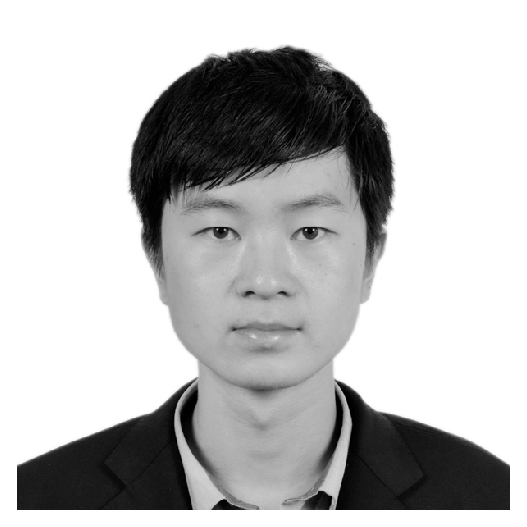
\includegraphics[width=1in,height=1.25in,clip,keepaspectratio]{./Authors/HaidongWang.eps}}]{Haidong Wang}
	 received the B.E. degree in Computer Science and Technology from Hunan University Of Technology and Business, Changsha, China, in 2014, and the M.Sc. degree in Computer Technology from the University of Chinese Academy of Sciences (UCAS), Beijing, 	China, in 2017. At present, he is currently pursuing the Ph.D. degree in Hunan University, Changsha, China. His current research interests include machine learning,  multi-object tracking and reinforcement learning.
\end{IEEEbiography}


%\begin{IEEEbiography}[{\includegraphics[width=1in,height=1.25in,clip,keepaspectratio]{./Authors/ZhiyongLi.eps}}]{Zhiyong Li}
%	received the MSc degree in System Engineering from National University of Defense Technology, Changsha, China, in 1996 and PhD degree in Control Theory and Control Engineering from Hunan University, Changsha, China, in 2004.
%	Since 2004, he joined the College of Computer Science and Electronic Engineering of Hunan University. 
%	Now, he is a Full Professor with Hunan University, member of IEEE, China Computer Federation (CCF) and Chinese Association for Artificial Intelligence (CAAI). 
%	His research interests include Intelligent Perception and Autonomous Moving Body, Machine Learning and Industrial Big Data, Intelligent Optimization Algorithms with Applications. He has published more than 100 papers in international journals and conferences.
%\end{IEEEbiography}
%
%
%\begin{IEEEbiography}[{\includegraphics[width=1in,height=1.25in,clip,keepaspectratio]{./Authors/XuanHe.eps}}]{Xuan He}
%	received her B.S. and M.S. degree from Hunan Normal University (HNU), China, in 2016 and 2020. She is currently pursuing the Ph.D. degree in Computer science and technology with Hunan  University. Her research interests include object detection and recognition, machine learning.
%\end{IEEEbiography}
%
%
%\begin{IEEEbiography}[{\includegraphics[width=1in,height=1.25in,clip,keepaspectratio]{./Authors/KeNai.eps}}]{Ke Nai}
%	received the Ph.D. degree in Computer Science and Technology from Hunan University, Changsha, China, in 2019. Currently, he is working as a Postdoctoral Researcher at Hunan University. His current research interests include visual tracking, face recognition, computer vision, pattern recognition and machine learning. He has published several papers in IEEE-TIP, Information Sciences, Knowledge Based Systems, Neural Computing and Applications, ICIP2019 and so on.
%\end{IEEEbiography}
%
%
%\begin{IEEEbiography}[{\includegraphics[width=1in,height=1.25in,clip,keepaspectratio]{./Authors/MingWen.eps}}]{Ming Wen}
%	 received his M.S. degree and Ph.D. degree from Hunan University in 2006 and 2010, respectively. He has been a senior engineer at State Grid Hunan Electric Power Company Limited Economical \& Technical Research Institute. His research interests include energy internet demand forecasting, electricity price, smart grid, renewable energy accommodation and power system planning.
%\end{IEEEbiography}


% that's all folks
\end{document}


% C#:  https://www.monodevelop.com/download/#fndtn-download-lin-ubuntu
